\documentclass[a4paper,12pt]{quantumarticle}
\pdfoutput=1

\usepackage{lipsum}

\title{Example use of rsmf}

\author{Johannes Jakob Meyer}

\begin{document}
\maketitle

\lipsum[1-3]

\begin{figure}
	\centering
	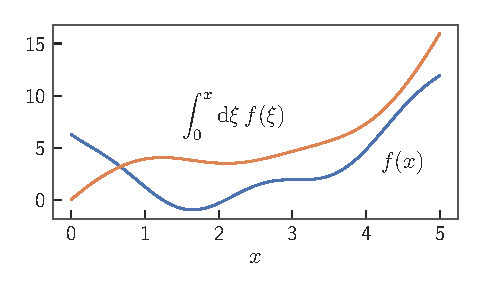
\includegraphics{annotated_plot}
	\caption{This is a very unfancy plot. But consider that both the size of the math formulas and the $x$ label are the same as in this caption (\texttt{small}). The axes labels are in a smaller fontsize, namely \texttt{footnotesize}: {\footnotesize 0.0}.}
\end{figure}

\lipsum[11-16]

\begin{figure*}
	\centering
	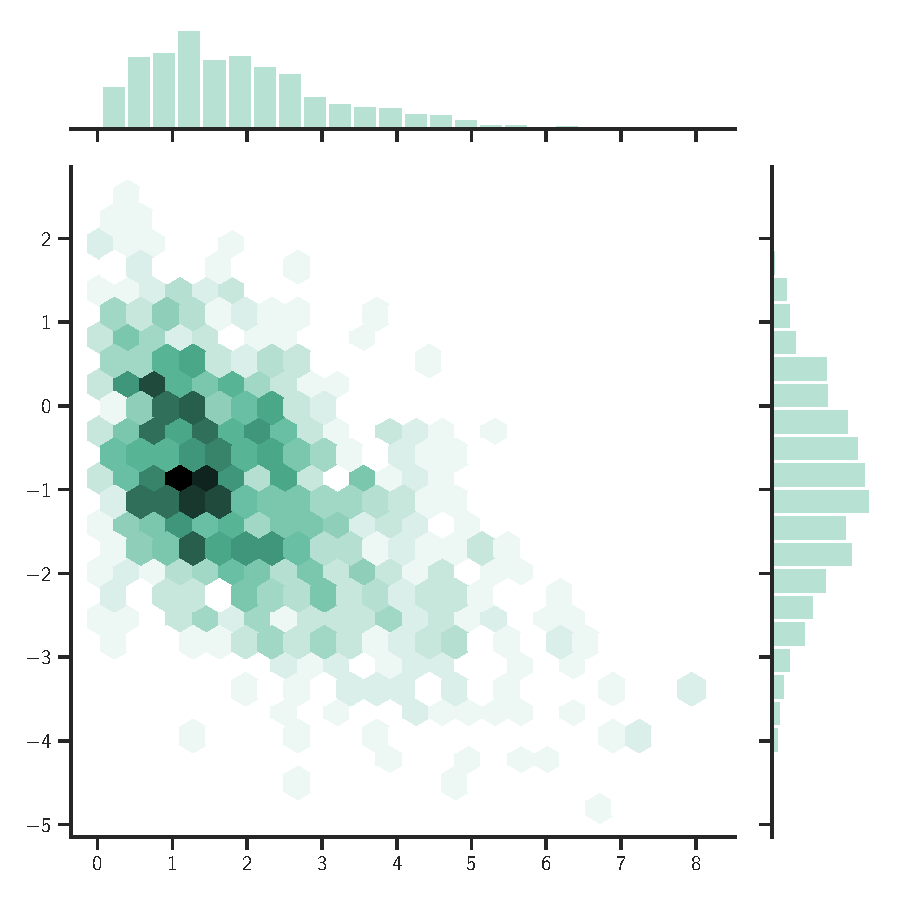
\includegraphics{hexbin}
	\caption{You can also use rsmf in conjunction with seaborn. Above you find an example plot from the seaborn gallery, again with matching fontsizes.}
\end{figure*}

\lipsum[11-16]

\begin{figure*}
\centering
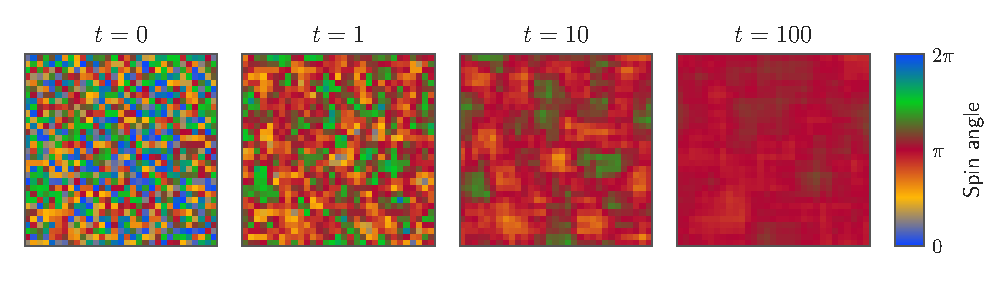
\includegraphics{spins}
\caption{Above is a more advanced example that contains multiple subplots.}
\end{figure*}

\lipsum[21-26]
    
\end{document}